\begin{figure*}[t]
  \begin{minipage}[t]{\textwidth}
    \centering
    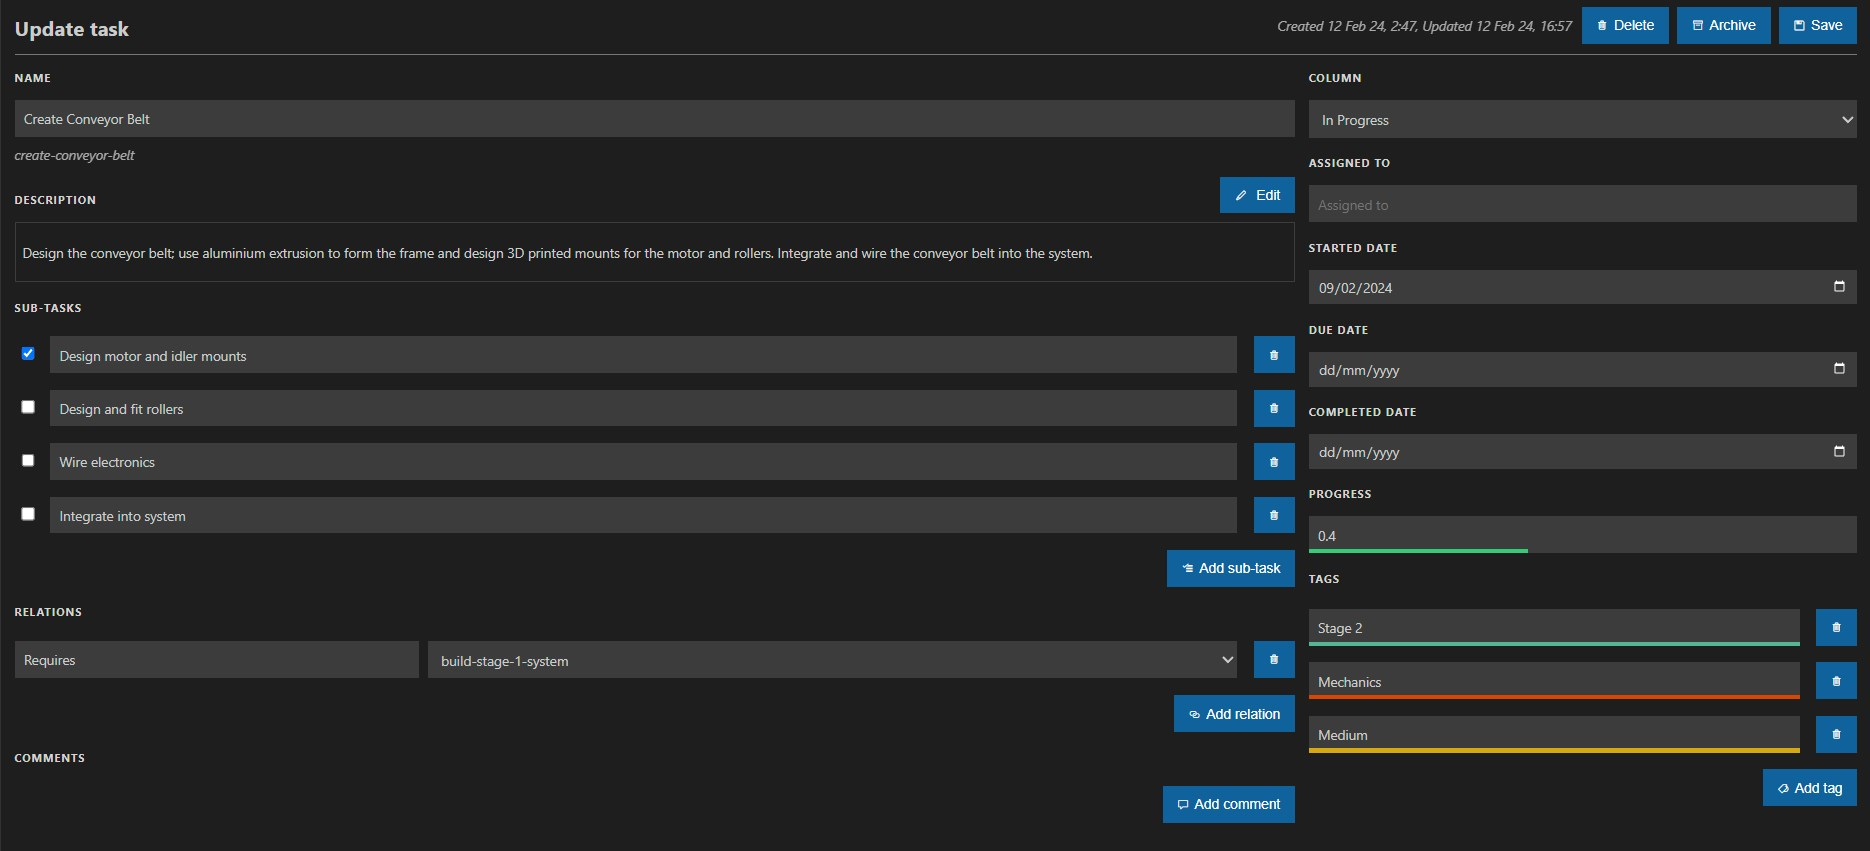
\includegraphics[width=\textwidth, height=\textheight, keepaspectratio]{imgs/appendix/taskexample.jpg}
    \caption{Example of Kanban Task}
    \label{fig:kantask}
  \end{minipage}
  \hfill 
\end{figure*}

\section{Project Plan}
\label{sec:projectplan}
For the planning of the project, the decision was made to leverage the experience gained from a 6-month placement by adopting more traditional software development methodologies.
This approach included the utilisation of a Kanban board to monitor the project's progress effectively.

In this Kanban board, labels were employed to categorise each task into different categories, such as
which component of the system the task is related to, the priority of the task, and the stage of the project the task is related to.
Each task had a description detailing what needed to be done, and some others had dependencies and checklists of sub-tasks that needed to be completed.
Dates were also assigned to each task to ensure that the project was on track. An example of a task on the Kanban board is shown in Figure \ref{fig:kantask},
detailing the task of developing the conveyor belt. A description of the task is given, as well as difficulty, workload, and the stage of the project it is related to.
There are also subtasks and dependencies listed, as well as the date the task was created and progress of the task.

\begin{figure*}[t]
  \begin{minipage}[t]{0.49\textwidth}
      \centering
      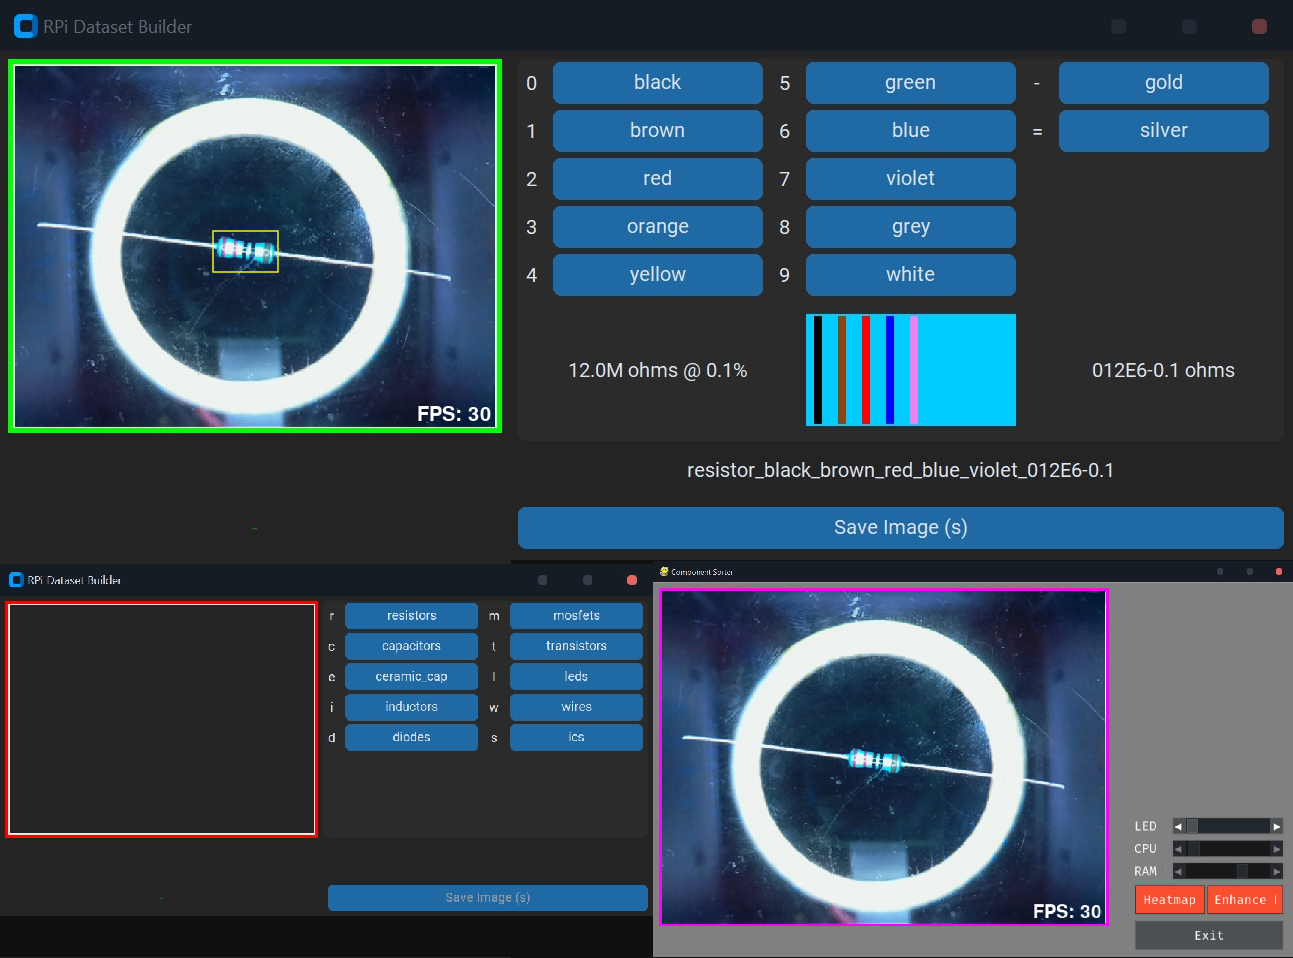
\includegraphics[width=\textwidth,height=6cm,keepaspectratio]{imgs/software/tools.png}
      \caption{Dataset Labeller Tool}
      \label{fig:customtool}
  \end{minipage}
  \hfill
  \begin{minipage}[t]{0.49\textwidth}
    \centering
    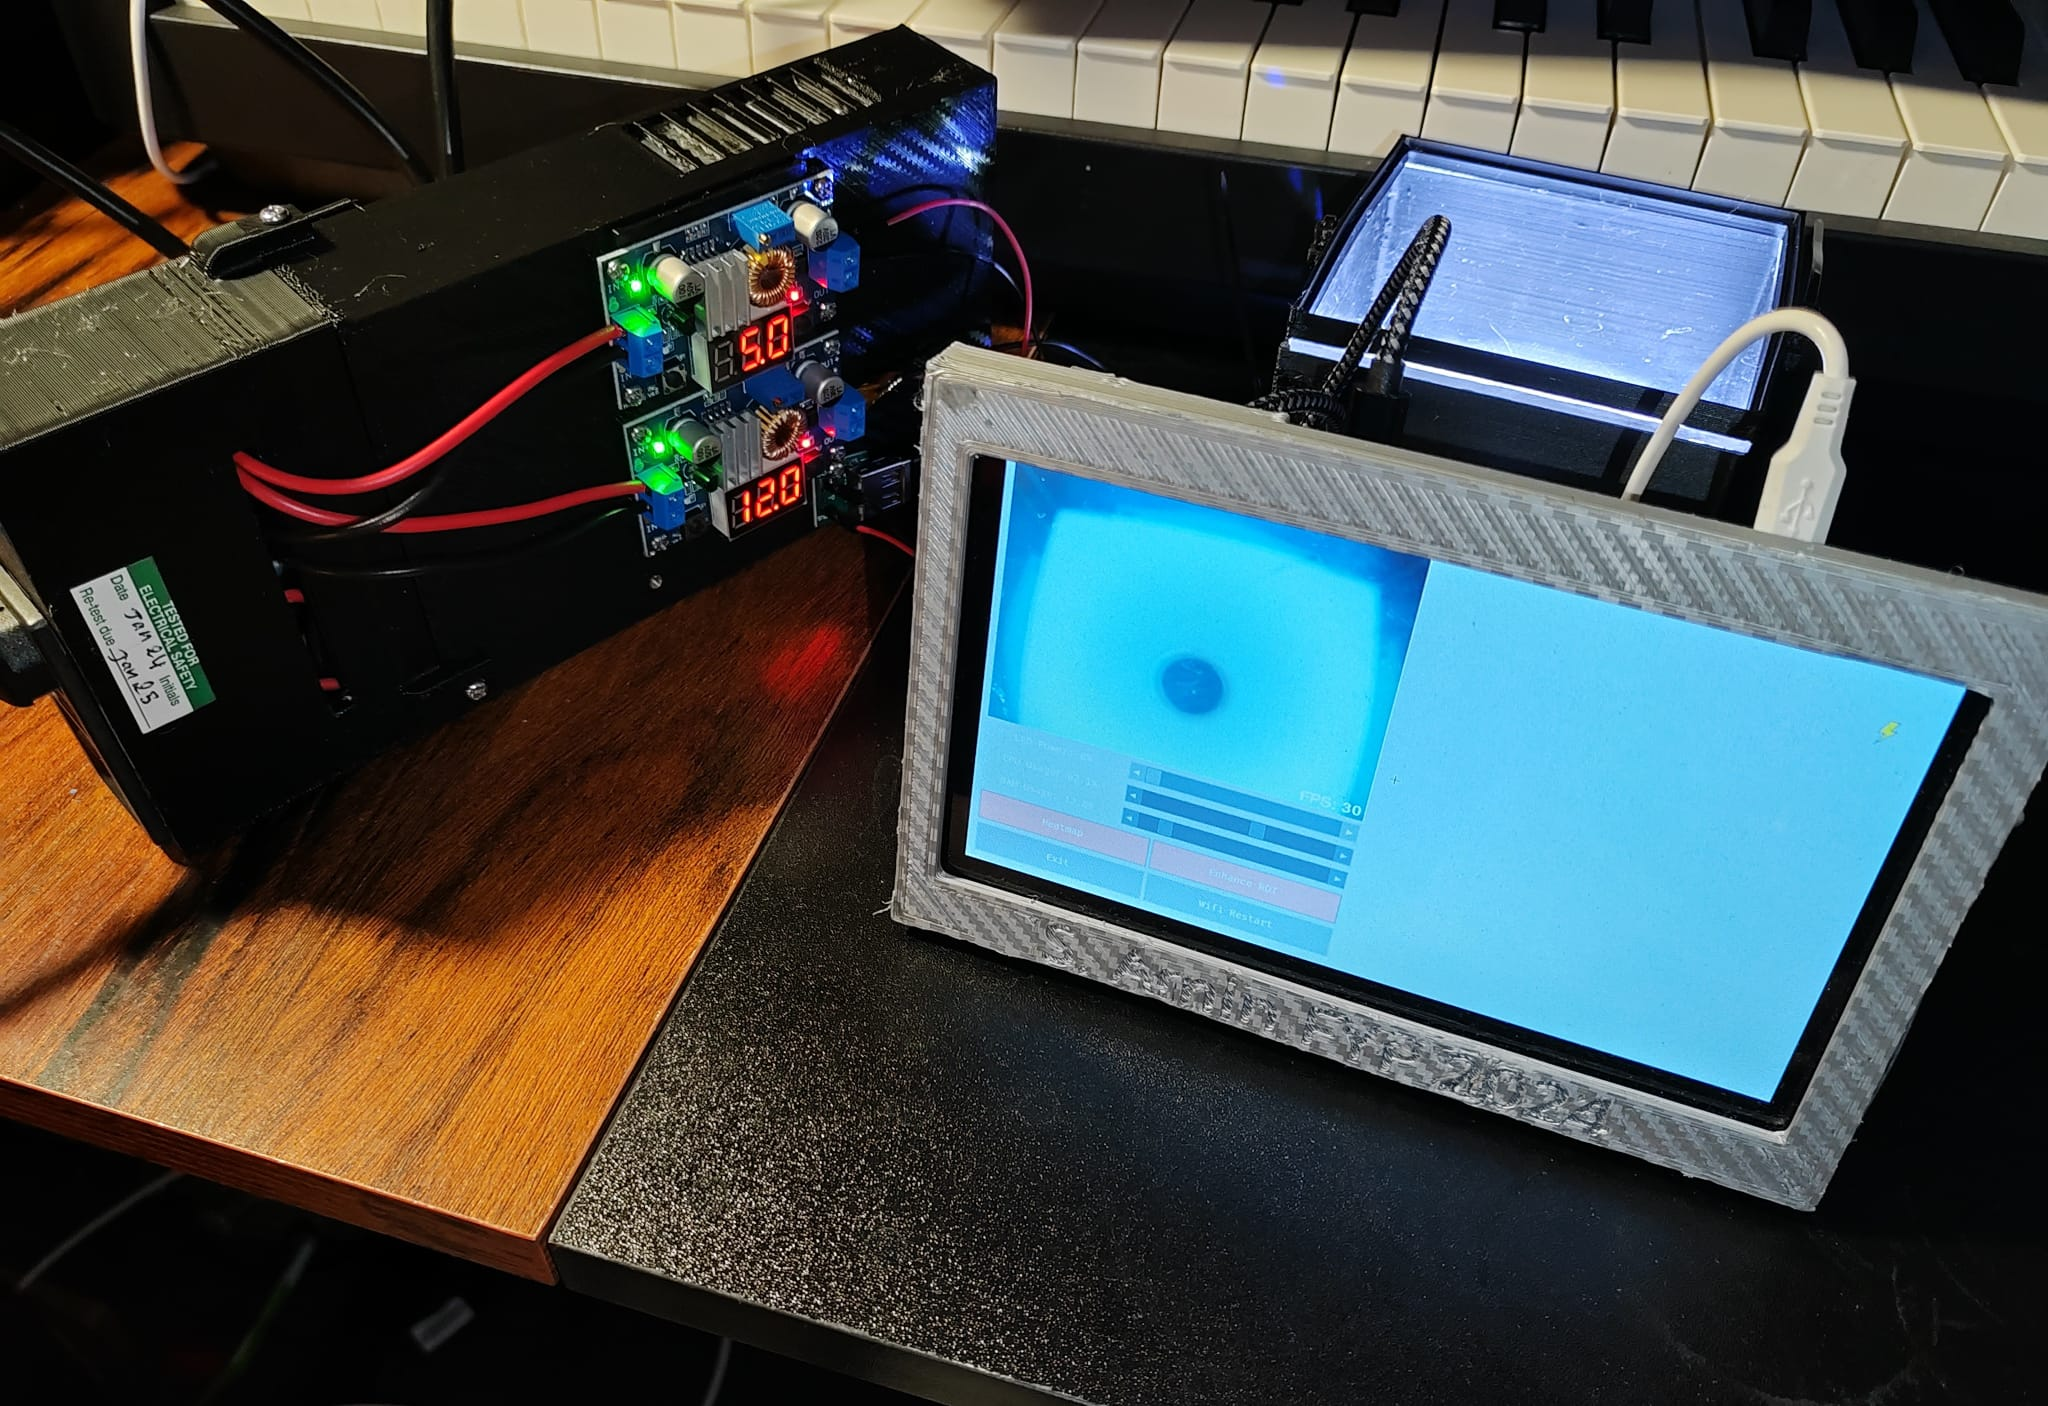
\includegraphics[width=\textwidth,height=6cm,keepaspectratio]{imgs/design/allparts.jpeg}
    \caption{Current System}
    \label{fig:allparts}
  \end{minipage}
  \hfill
\end{figure*}

\noindent
The main labels used in the Kanban board are as follows:
\begin{mylist}
  \item \textbf{Stage} \\
  This label is used to categorise the task into the stage of the project it is related to. The stages are as follows:
  \begin{multicols}{2}
    \vspace{-0.5em} 
    \begin{mylist}
      \item Stage 1
      \item Stage 2
      \item Stage 3
      \item Stage 4
    \end{mylist}
    \vspace{-0.5em} 
  \end{multicols}
  \item \textbf{Component} \\
  This label is used to categorise the task into the component of the system it is related to. The components are as follows:
  \begin{mylist}
    \item HME (Hardware, Mechanics, Electronics)
    \item Vision
    \item Logistics
    \item Software
  \end{mylist}
  \item \textbf{Workload} \\
  This label is used to categorise the task based on the expected workload. The workloads are as follows:
  \begin{multicols}{2}
    \vspace{-0.5em} 
    \begin{mylist}
      \item Trivial (0)
      \item Tiny (1)
      \item Small (2)
      \item Medium (3)
      \item Large (5)
      \item Huge (8)
    \end{mylist}
    \vspace{-0.5em} 
  \end{multicols}
\end{mylist}

For the remainder of the project, this Kanban board will be used to track the progress of the project. 

As mentioned previously, to keep track of the components of the system, a spreadsheet was maintained which is shown in Appendix \ref{app:bom}.
\subsection{Stage 1}
The original plan for Stage 1 was to develop a system that could identify and classify components. However, the development 
of the foundation and hardware, as well as software to control the hardware, took longer than expected. This was because
the vision system needed to be trained on data that is representative of the conditions it will be used in, which 
required the mechanical design to be finalised, and can be seen from the dependencies listed on the Kanban board in Figure \ref{fig:projectplan}.
As such, Stage 1 was split into two stages, with the first stage focusing on the development of the foundation of the system, and the second stage focusing on the development of the computer vision system.

While non-trivial, the strong foundation of the project instills confidence that Stage 2 can be accomplished within the next 5-6 weeks.
The current Stage 1 system is shown in Figure \ref{fig:allparts} and the system diagram is shown in Figure \ref{fig:sysdiagram}.
This diagram clearly shows the interdependency of all the components of the system, and how the development of the hardware is a prerequisite for the development of the software.
This further reinforces the need to underpin the project with a strong, modular and parallel development approach.

\subsection{Stage 2}
For the Stage 2 system, the system will be able to identify and classify components. 
The main tasks for this stage are as follows:
\begin{mylist}
    \item \textbf{Conveyor Belt System} \\
    A conveyor belt system will be developed to move the components from the input to the vision system.
    \item \textbf{Component Classification} \\
    The system will need to be able to classify the components. This will be done using a YOLOv8 model, which will be trained on a dataset of components.
    \item \textbf{Component Value Identification} \\
    After the component has been classified, the system will need to identify the value of the component. This will be done by using
    a separate model to identify the value of the component. In particular, the model for the resistors will be the highest
    priority given their complexity, followed by text-based values for capacitors and inductors, and finally ICs and MOSFETs.
    \item \textbf{User Interface} \\
    The UI of the system will need to be updated to reflect the system's new functionality. This will be done using the Pygame library\cite{pygamedoc}.
\end{mylist}

\subsection{Stage 3}
For the Stage 3 system, the system will become semi-autonomous, with the user having to manually place the components into the system, and the system
automatically sorting the components into the correct bins after classifying and identifying the components. 

For the Stage 3 system, the following tasks will need to be completed:
\begin{mylist}
    \item \textbf{Sorting Mechanism} \\
    The system will need to be able to sort the components into the correct bins. This will be done using a servo motor to move the components into the correct bin.
    This not only requires the software to be developed but also the physical mechanism to be designed and built, including the bins themselves.
    This is a non-trivial task, and so will be the main focus of this stage.
    \item \textbf{User Interface} \\
    The UI of the system will need to be updated to reflect the system's new functionality. This will be done using the Pygame library\cite{pygamedoc}.
\end{mylist}

\subsection{Stage 4}
The final stage of the system will be to make the system fully autonomous, with the system being able to identify and sort components without any user input.
The main task for this stage will be to develop a device that can automatically feed the components into the system, and as 
discussed in Section \ref{sec:background} (Background), this will likely be done with a vibratory bowl feeder (VBF).

Ensuring system reliability will also be a key task for this stage, as at this point the system will contain many moving parts, and will need to be able to
operate reliably for extended periods. This stage will mostly involve fine-tuning the system and logistics such as
finalising the final report and presentation.

\noindent
In terms of time management, the decision to enroll in only two modules this term was made after opting to complete four modules in the first term. Substantial work has already been completed
during the Christmas break, so there is confidence that sufficient time on the project can be spent during this Spring term.

\begin{figure*}[t]
  \begin{minipage}[t]{0.49\textwidth}
      \centering
      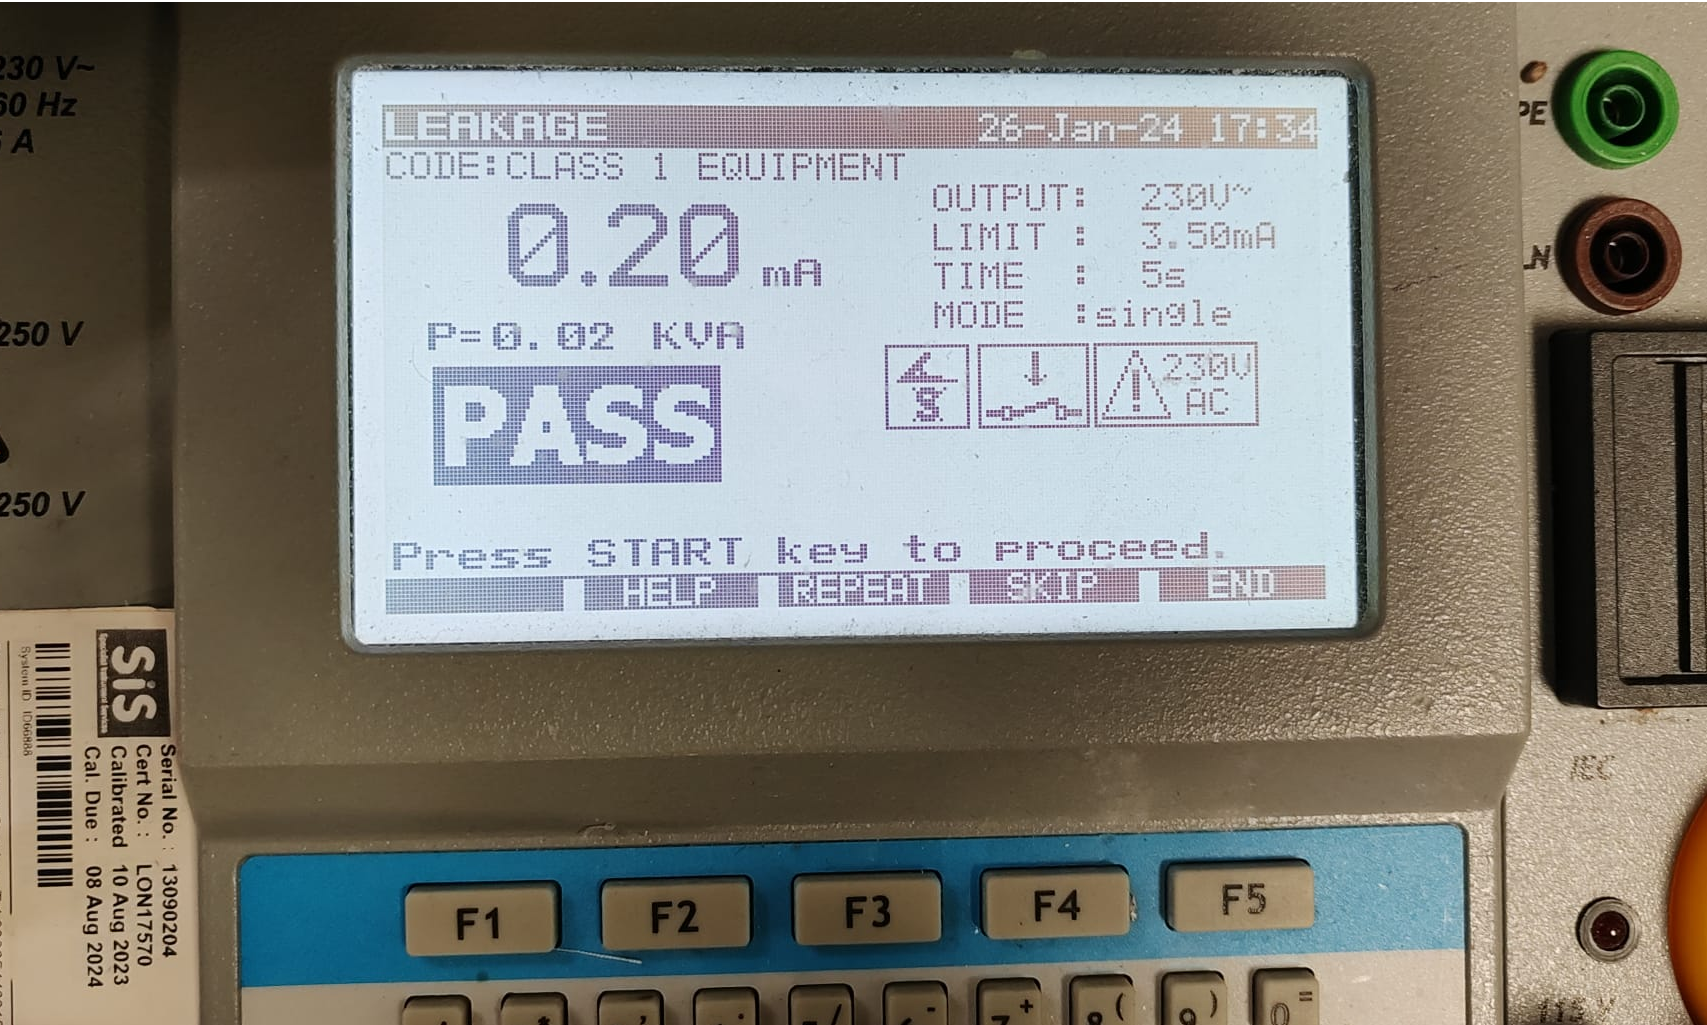
\includegraphics[width=\textwidth,height=7cm, keepaspectratio]{imgs/pattesting.jpeg}
      \caption{PAT Testing Machine}
      \label{fig:pat}
    \end{minipage}
    \hfill
    \begin{minipage}[t]{0.49\textwidth}
      \centering
      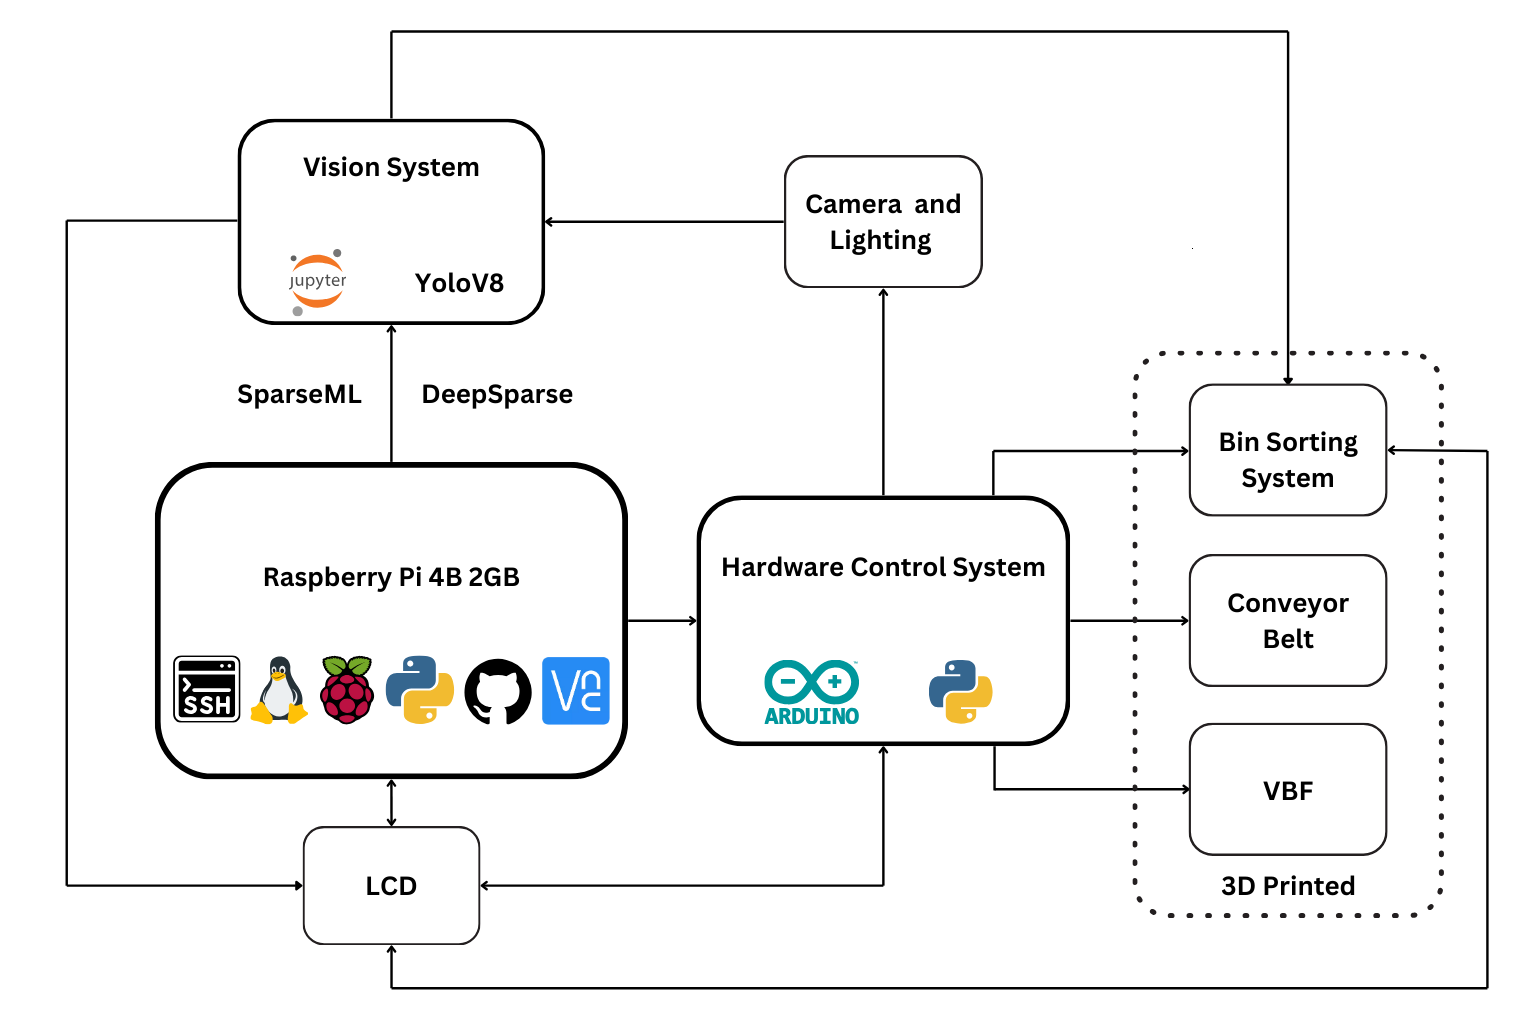
\includegraphics[width=\textwidth,height=7cm, keepaspectratio]{imgs/diagrams/systemdiagram.png}
      \caption{Stage 1 System Diagram}
      \label{fig:sysdiagram}
    \end{minipage}
    \hfill
\end{figure*}

\subsection{Fallbacks and Extensions}
Although extensive planning has been completed, it is important to consider potential fallbacks and extensions.

A major fallback would be if the system is unable to identify and classify the components in real-time, thus making
the system slower than the current manual process. This would be mitigated by a fully autonomous system, however
depending on the degree of human intervention required, the system may not be viable for its intended purpose. The solution
to this would be to develop a much more capable model deployed on a more powerful device, such as a cloud server, which would
be able to process the video feed in real-time. This would only require retraining a higher capacity model, so would not be a cause for 
concern, however, some additional time would be required to develop the cloud server and the communication between the server and the system.

Another potential fallback is the low accuracy of the computer vision system. This would require retraining the model with a larger dataset, and 
potentially employing more advanced computer vision techniques or by using a new model entirely. Depending on the extent of the issue, this could
be a significant setback, however, the system has been designed in such a way that the computer vision system can be easily replaced, so this should be somewhat mitigated.

Another potential fallback is the mechanical failure of any of the components of the system. This would be mitigated by having spares of the most critical components,
and ensuring that the system is designed in such a way that the components can be easily replaced. This was considered in the design of the system, and so
should not be a major issue if it occurs. The choice of using PLA for the 3D printed parts may be a potential issue, as it is known
to be susceptible to warping and degradation over time, however, the parts are not under extreme mechanical stress, and so may not be an issue. Extensive
stress testing will be conducted to ensure that the parts are reliable.

An extension to the project would be to allow IC testing and sorting. This would require a new model to be developed to identify the ICs, and a new sorting mechanism to be developed to sort the ICs.
This would be a large extension to the project, and so would require a significant amount of additional time to complete, however, it would be a valuable extension to the project, as it would reduce the amount of waste generated by the department.
The autonomous implementation of this would likely involve the use of a robotic arm to pick up the ICs to test them, but a simpler approach could be to have the user place
the ICs into a tester manually, and then the system would sort the ICs based on the results of the test.

In the same vein, another extension to the project would be to allow the system to test the components. This requires much more fine-tuned control of the components, namely
the ability to correctly orient the components and to apply the correct voltage and current to the component.
This would be an incredible extension to the project, and so would require a significant amount of additional time to complete, however, it would be a valuable extension to the project, as it would allow the department to reuse components that are still functional, and would reduce the amount of waste generated by the department.